\section{系统需求分析}

\subsection{项目目标}
本项目的目标是从零实现一个科学计算器,支持实数与分数的四则运算以及常见函数运算,并提供可视化交互界面。
计算器的详细功能如下:

\begin{enumerate}
    \item 实数与实数、实数与分数、分数与分数的加、减、乘、除运算。
    \item 通过括号控制运算优先级。
    \item 常用函数,包括阶乘、幂函数、开方、倒数、三角函数、对数函数。
    \item 提供常用的矩阵运算操作,包括矩阵的加法、减法、乘法。
    \item 提供数据库连接,并对数据进行描述性统计,保存统计数据。
\end{enumerate}

总之,本计算器最终的目标是实现覆盖当前手机自带计算器的所有功能,并另外集成矩阵与数据库的操作,并且方便使用。

\subsection{功能说明}

\begin{figure}[!htbp]
    \centering
    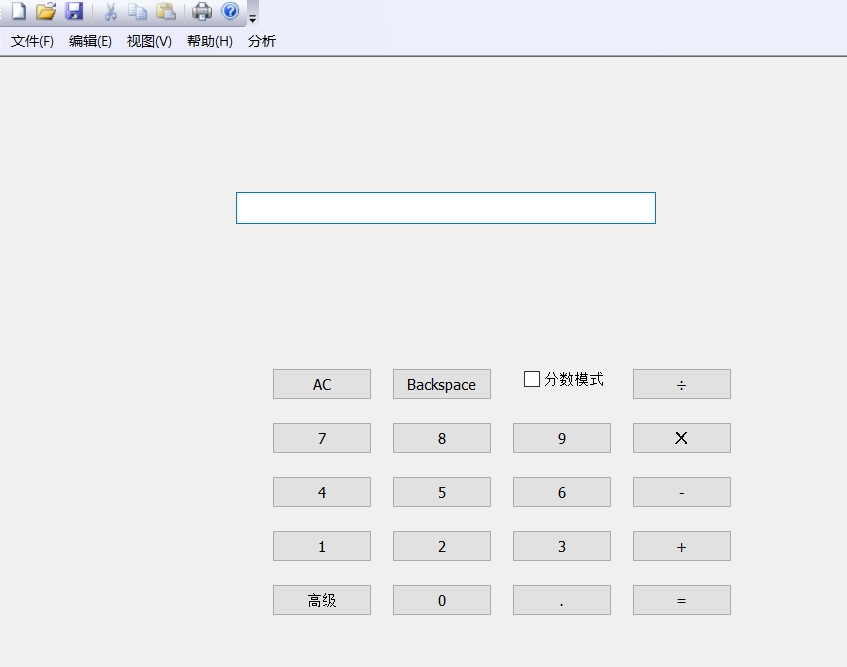
\includegraphics[width = 12cm]{MainPage.jpg}
    \caption{主界面}
    \label{fig:Dialog}
\end{figure}
计算器的基本界面如\autoref{fig:Dialog}所示,设计仿照现代手机自带的计算器,基础使用方法完全相同,
用户通过点击对应按钮向编辑框中输入算式,点击“=”,可以计算并把结果显示在编辑框。
勾选“分数模式”,可以输入分数,并且运算结果也都用分数表示
(此处的分数四则运算不是浮点数的近似表示,而是完全精确的)。

\begin{figure}[!htbp]
    \centering
    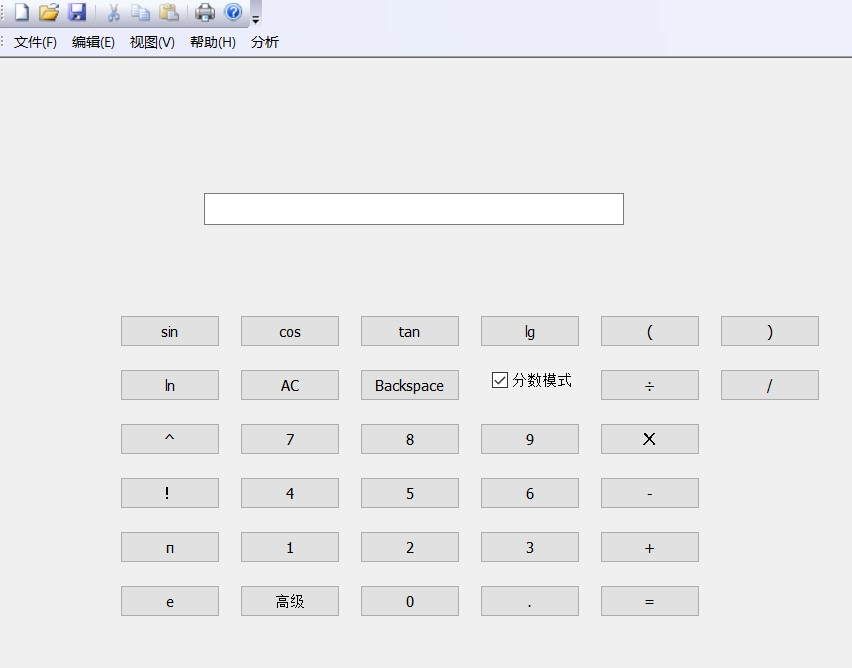
\includegraphics[width = 12cm]{高级.jpg}
    \caption{高级主界面}
    \label{fig:Advance}
\end{figure}
如果点击“高级”,则会显示常用的科学计算符号,如\autoref{fig:Advance}所示。

\begin{figure}[!htbp]
    \centering
    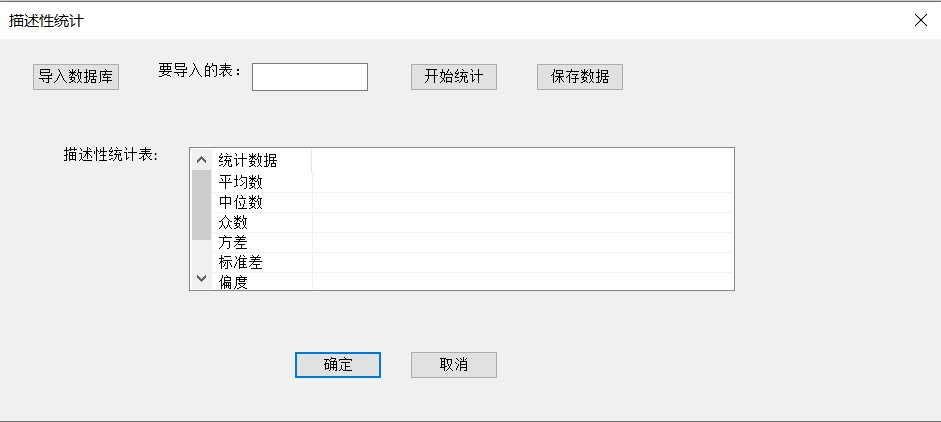
\includegraphics[width = 12cm]{描述性统计.jpg}
    \caption{描述性统计界面}
    \label{fig:DesStat}
\end{figure}
\begin{figure}[!htbp]
    \centering
    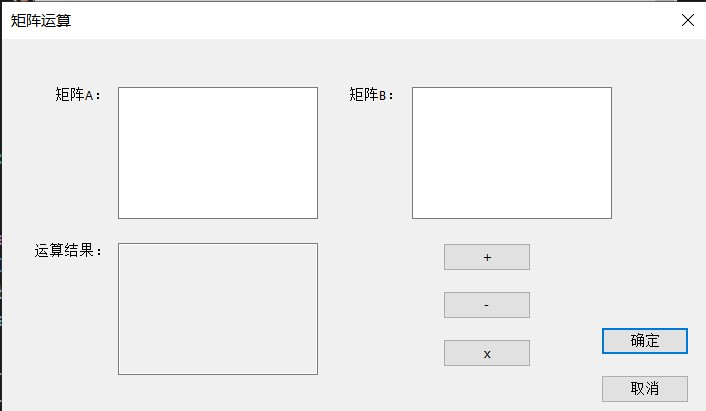
\includegraphics[width = 12cm]{矩阵运算.jpg}
    \caption{矩阵运算界面}
    \label{fig:MatrixManip}
\end{figure}
在菜单栏,提供了“高级”选项,可以选择“描述性统计”或“矩阵运算”,点击后会弹出相应对话框,如\autoref{fig:DesStat} 和 
\autoref{fig:MatrixManip}所示。
   
在“描述性统计”中,点击导入数据库,会打开文件浏览窗口;选择数据库文件后,填写
要统计的表,点击“开始统计”,
程序以每列作为一个指标,计算各列的描述统计数据,包括平均数、中位数、众数、
方差、标准差、偏度、峰度(自动忽略第一列ID),点击“保存数据”,可以保存至txt文件。

在“矩阵运算”中,以空格分隔行向量中不同数据,以换行分隔不同行向量;点击相应按钮得到计算结果。